\setNextFileName{ClassAndCodeManagement.html}
\begin{section}{Class and Code Management}
\label{sec:classandcodemanagement}

The runtime maintains a database of Java instances which identifies the currently loaded class and method base. The classloader class base enables the runtime to identify and dynamically load undefined classes as they required during execution. All the classes, methods and compiled code arrays required to enable the runtime to operate are pre-installed in the initial boot image. Other runtime classes and application classes are loaded dynamically as they are needed during execution and have their methods compiled lazily. The runtime can also identify the latest compiled code array (and, on occasions, previously generated versions of compiled code) of any given method via this classbase and recompile it dynamically should it wish to do so.

Lazy method compilation postpones compilation of a dynamically loaded class' methods at load-time, enabling partial loading of the class base to occur. Immediate compilation of all methods would require loading of all classes mentioned in the bytecode in order to verify that they were being used correctly. Immediate compilation of these class' methods would require yet more loading and so on until the whole classbase was installed. Lazy compilation delays this recursive class loading process by postponing compilation of a method until it is first called.

Lazy compilation works by generating a stub for each of a class' methods when the class is loaded. If the method is an instance method this stub is installed in the appropriate TIB slot. If the method is static it is placed in a linker table located in the JTOC (linker table slots are allocated for each static method when a class is dynamically loaded). When the stub is invoked it calls the compiler to compile the method for real and then jumps into the relevant code to complete the call. The compiler ensures that the relevant TIB slot/linker table slot is updated with the new compiled code array. It also handles any race conditions caused by concurrent calls to the dummy method code ensuring that only one caller proceeds with the compilation and other callers wait for the resulting compiled code.

\begin{subsection}{Class Loading}

Jikes\textsuperscript{TM} RVM implements the Java\textsuperscript{TM} programming language's dynamic class loading. While a class is being loaded it can be in one of seven states. These are:
\begin{itemize}
  \item \textbf{vacant}: The \spverb+RVMClass+ object for this class has been created and registered and is in the process of being loaded.
  \item \textbf{loaded}: The class's bytecode file has been read and parsed successfully. The modifiers and attributes for the fields have been loaded and the constant pool has been constructed. The class's superclass (if any) and superinterfaces have been loaded as well.
  \item \textbf{resolved}: The superclass and superinterfaces of this class has been resolved. The offsets (whether in the object itself, the JTOC, or the class's TIB) of its fields and methods have been calculated.
  \item \textbf{instantiated}: The superclass has been instantiated and pointers to the compiled methods or lazy compilation stubs have been inserted into the JTOC (for static methods) and the TIB (for virtual methods).
  \item \textbf{initializing}: The superclass has been initialized and the class initializer is being run.
  \item \textbf{initialized}: The superclass has been initialized and the class initializer has been run.
  \item \textbf{class initializer has failed}: There was an exception during execution of the \spverb+<clinit>+ method so the class cannot be initialized successfully.
\end{itemize}

\end{subsection}

\begin{subsection}{Code Management}

A compiled method body is an array of machine instructions (stored as ints on PowerPC\textsuperscript{TM} and bytes on x86-32). The Jikes RVM Table of Contents(JTOC), stores pointers to static fields and methods. However, pointers for instance fields and instance methods are stored in the receiver class's \hyperref[sec:objectmodel]{TIB}. Consequently, the dispatch mechanism differs between static methods and instance methods.

\begin{subsubsection}{The JTOC}

The JTOC holds pointers to each of Jikes\textsuperscript{TM} RVM's global data structures, as well as literals, numeric constants and references to String constants. The JTOC also contains references to the TIB for each class in the system. Since these structures can have many types and the JTOC is declared to be an array of ints, Jikes RVM uses a descriptor array, co-indexed with the JTOC, to identify the entries containing references. The JTOC is depicted in the figure below.

\begin{figure}[h]
  \centering
  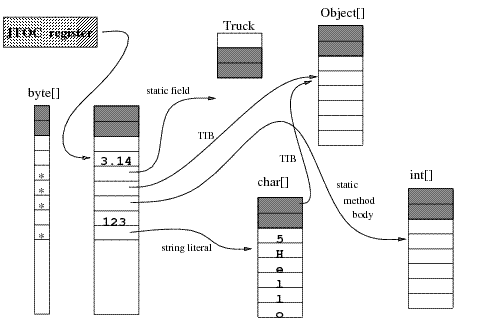
\includegraphics[width=\linewidth]{images/ClassAndCodeManagement-JTOC.png}
\end{figure}

\end{subsubsection}

\begin{subsubsection}{Virtual Methods}

A TIB contains pointers to the compiled method bodies (executable code) for the virtual methods and other instance methods of its class. Thus, the TIB serves as Jikes RVM's virtual method table. A virtual method dispatch entails loading the TIB pointer from the object reference, loading the address of the method body at a given offset off the TIB pointer, and making an indirect branch and link to it. A virtual method is dispatched to with the invokevirtual bytecode; other instance methods are invoked by the invokespecial bytecode.

\end{subsubsection}

\begin{subsubsection}{Static Fields and Methods}

Static fields and pointers to static method bodies are stored in the JTOC. Static method dispatch is simpler than virtual dispatch, since a well-known JTOC entry method holds the address of the compiled method body.

\end{subsubsection}

\begin{subsubsection}{Instance Initialization Methods}

Pointers to the bodies of instance initialization methods, \spverb+<init>+, are stored in the JTOC. (They are always dispatched to with the \spverb+invokespecial+ bytecode.)

\end{subsubsection}

\begin{subsubsection}{Lazy Method Compilation}

Method slots in a TIB or the JTOC may hold either a pointer to the compiled code, or a pointer to the compiled code of the \textit{lazy method invocation stub}. When invoked, the lazy method invocation stub compiles the method, installs a pointer to the compiled code in the appropriate TIB or the JTOC slot, then jumps to the start of the compiled code.

\end{subsubsection}

\begin{subsubsection}{Interface Methods}

Regardless of whether or not a virtual method is overridden, virtual method dispatch is still simple since the method will occupy the same TIB offset its defining class and in every sub-class. However, a method invoked through an \spverb+invokeinterface+ call rather than an \spverb+invokevirtual+ call, will not occupy the same TIB offset in every class that implements its interface. This complicates dispatch for \spverb+invokeinterface+.

The simplest, and least efficient way, of locating an interface method is to search all the virtual method entries in the TIB finding a match. Instead, Jikes RVM uses an \textit{Interface Method Table (IMT)} which resembles a virtual method table for interface methods. Any method that could be an interface method has a fixed offset into the IMT just as with the TIB. However, unlike in the TIB, two different methods may share the same offset into the IMT. In this case, a \textit{conflict resolution stub} is inserted in the IMT. Conflict resolution stubs are custom-generated machine code sequences that test the value of a hidden parameter to dispatch to the desired interface method. For more details, see \spverb+InterfaceInvocation+.

\end{subsubsection}

\end{subsection}

\end{section}
